\begin{evenBlock}{Block Passing}

\begin{minipage}[t]{\linewidth}
    \centering
    
    \begin{minipage}{.4\linewidth} % Left column and width
        \centering
        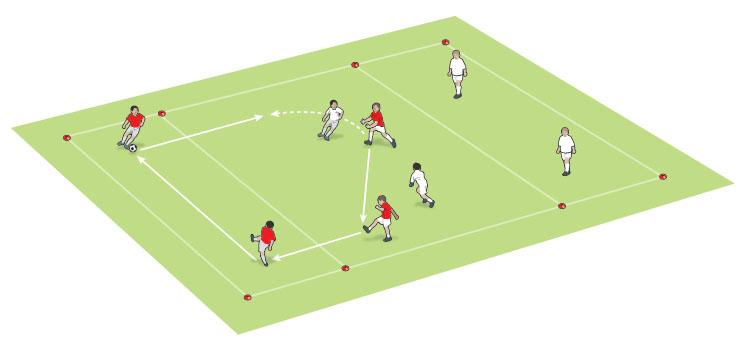
\includegraphics[width=\textwidth]{../img/Trimmed/Block_Passing_1}
        \vspace{6pt}
        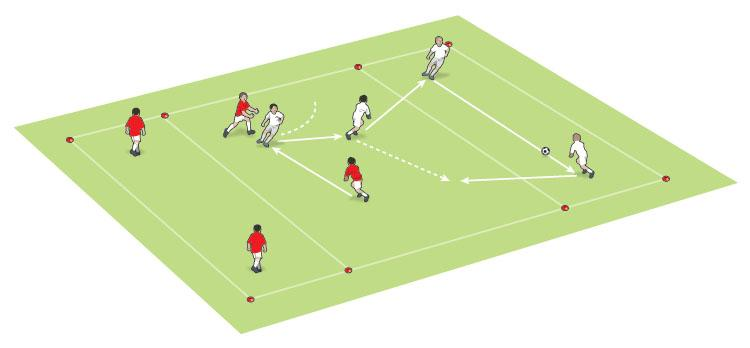
\includegraphics[width=\textwidth]{../img/Trimmed/Block_Passing_2}
    \end{minipage}
    \hspace{0.05\linewidth}
    \begin{minipage}{.5\linewidth} % Left column and width
        \textbf{Drill Description:}
        A drill that focuses on pressing and avoiding the press.  The goal is to keep the ball as long as possible.
        
        \begin{enumerate}
        \setlength{\itemsep}{0pt}
        \setlength{\parskip}{0pt}
        \setlength{\parsep}{0pt}
        \item This is a 4v4 game.
        \item 20x15 yard area with two 5 yard end zones.
        \item The end zones are safe zones and are occupied with 2 teammates.
        \item The other 2 teammates from each team are in the central zone playing 2v2 keep away.
        \item The center players can pass to the end zone players who are safe from attack, but only after they successully passed it within the central zone.
        \end{enumerate}

        \textbf{Coaching Points:}
        \begin{enumerate}
        \setlength{\itemsep}{0pt}
        \setlength{\parskip}{0pt}
        \setlength{\parsep}{0pt}
        \item Where are you passing options?
        \item Support your teammate.
        \item Know where the ball is!
        \item Block the ball or the pass.  Know where your team is.
        \item Without the ball move and talk so your partner knows where you are without seeing you.
        \end{enumerate}
    \end{minipage}
\end{minipage}

\end{evenBlock}